\chapter{Diferentes implementaciones de k-Means}

\section{Lloyd's K-Means}
El \textbf{algoritmo de Lloyd} es el comúnmente conocido como algoritmo \textbf{K-Means} que particiona un conjunto de datos en $K$ clústeres. Los pasos del algoritmo son los siguientes:

\begin{enumerate}
    \item Inicializa los centroides.
    \item En cada iteración:
    \begin{itemize}
        \item Asigna un punto al clúster más cercano.
        \item Calcula nuevos centroides.
        \item Verifica si los centroides han cambiado significativamente (convergencia).
    \end{itemize}

    \item Finaliza cuando los centroides ya no cambian significativamente o se alcanza el número máximo de iteraciones.

    
\end{enumerate}



\section{MacQueen's K-Means}
El problema de Lloyd's es que cuando actualiza las asignaciones de puntos de datos a clústeres, no actualiza los centroides. No tiene en cuenta que con cada actualización, el centroide cambia de posición y puede suponer que un punto esté erróneamente asignado a un centroide porque no fue actualizado.

MacQueen intenta solventar este problema actualizando los centroides con cada nueva asignación lo que también supone más tiempo de cálculo. El proceso es similar al de Lloyd's, solo que se vuelven a calcular los centroides asignados:

\begin{enumerate}
    \item Inicialización de los centroides: se comienza seleccionando aleatoriamente $K$ puntos como centroides iniciales.

    \item Asignación de puntos a centroides de manera secuencial: se calcula la distancia (euclidiana) entre cada punto del dataset y cada uno de los centroides. Se asigna el punto al centroide más cercano.

    \item Se recalculan los centroides de los clústeres después de cada asignación.

    \item Repetición: los pasos de asignación de centroides y de actualización de de estos se repiten iterativamente hasta que se converja o se alcance un número máximo de iteraciones.

    \item Convergencia.
\end{enumerate}

Diferencias entre Lloyd's y MacQueen's:

\begin{itemize}
    \item Lloyd's actualiza los centroides en pasos discretos, recalculándolos después de asignar todos los puntos de datos. Esto es más eficiente ya que se las actualizaciones se generan en un solo instante, pero requiere más iteraciones para converger debido a los cambios de centroides en cada iteración.

    \item MacQueen's actualiza los centroides de manera continua, cada vez que se asigna un punto de datos, lo que garantiza la correcta asignación del punto a un grupo de datos. Es menos eficiente que Lloyd's si estamos frente a un gran conjunto de datos, pero mejor si el flujo de datos es continuo. Converge más rápido, ya que el número de iteraciones se ajustan continuamente a los centroides.
\end{itemize}



\section{Hartigan-Wong K-Means}
Los algoritmos anteriores escogen los centroides iniciales de manera no eficiente y puede que no converja a causa de una mala inicialización.

El algoritmo de Hartigan-Wong asigna los puntos de datos a los centroides de forma aleatoria. Luego, se calcula cada centroide como la media de los puntos asignados. Así, no asocio un punto al centroide más cercano, sino al que mejor inercia da.


\begin{enumerate}
    \item Inicialización de centroides: seleccionar aleatoriamente K puntos como centroides iniciales.

    \item Al azar se asignan los puntos a un centroide.

    \item Se calcula el centroide como la media de los puntos asignados.

    \item Se repite hasta la convergencia o hasta el número máximo de iteraciones.
\end{enumerate}

\subsubsection{Diferencias entre Hartigan-Wong y Lloyd's K-Means}

\begin{itemize}
    \item En términos computacionales, Lloyd's es más simple y menos complejo que Hartigan-Wong.

    \item Hartigan-Wong requiere menos iteraciones para converger, ya que optimiza de manera continua las ubicaciones de los puntos (las actualizaciones de centroides son más frecuentes y locales al considerar la reubicación de puntos entre grupos durante las iteraciones).
\end{itemize}



\section{Elkan's K-Means}
El algoritmo de Elkan se diseñó para acelerar la convergencia de K-Means y reducir el número de cálculos de distancia necesarios. Sus principios son los siguientes:

\begin{itemize}
    \item Reducción de cálculos de distancia: Elkan utiliza los límites superiores e interiores. Elkan se basa en que si sabemos que un punto está cerca de un centroide particular, podemos evitar calcular la distancia de ese punto a otros centroides lejanos.

    \item Desigualdad triangular: evitamos calcular distancias innecesarias. La desigualdad triangular establece que, para cualquier triángulo, la suma de las longitudes de dos de sus lados será mayor o igual que la longitud del tercer lado.

    \item Actualización eficiente: cada vez que los centroides se actualizan, los límites superiores e inferiores también lo hacen, minimizando cálculos futuros.
\end{itemize}

\begin{enumerate}
    \item Inicializar los centroides de los k clústeres.

    \item Mantener un límite superior e inferior de las distancias de cada punto a los centroides. Así evitamos cálculos de distancias innecesarios.

    \item Usamos estos límites para determinar el clúster más cercano a cada punto de datos sin calcular todas las distancias.

    \item Asignar cada punto al clúster más cercano.

    \item Actualizar los centroides: calcular nuevos centroides basado en las asignaciones actuales de los puntos a los grupos.

    \item Actualización de límites: actualizar los límites superiores e inferiores tras mover los centroides.

    \item Iteración: repetir los pasos 2 a 5 hasta que se alcance la convergencia o se alcance un número máximo de iteraciones.


\end{enumerate}

\begin{itemize}
    \item Ventajas: reduce el número de cálculos de distancia.
    \item Ventajas: escalabilidad en grandes conjuntos de datos debido a la optimización de cálculos de distancia.

    \item Limitaciones: complejo de implementar.
    \item Limitaciones: sensible a la inicialización de los centroides.
\end{itemize}


\section{Soft K-Means / Fuzzy K-Means}
Uno de los grandes problemas de K-Means es su sensibilidad a la hora de inicializar los centroides. Esto se puede solventar inicializando K-Means varias veces y utilizar el valor que mejor separe a los grupos. \textbf{Soft K-Means} (o \textbf{Fuzzy K-Means}) permite que los datos pertenezcan parcialmente a múltiples grupos, en lugar de asignar cada punto estrictamente a un único grupo.

Pasos del algoritmo Soft K-Means:

\begin{enumerate}
    \item Inicialización: selección de $k$ centroides iniciales. Para cada punto $p$, se aplica una función de membresía $u$ entre 0 y 1 que indica que tan alejado/cerca está el punto $p$ del centroide del grupo. La suma de los valores de $u$ para cada punto $p$ debe ser $1$ ya que es la suma de probabilidades.

    \item Actualización de los centroides: Calculamos los centroides $C_1$ y $C_2$ en función de los valores de pertenencia. El valor centroide $C_j$ se actualiza de la siguiente manera:
    \begin{equation*}
        C_j= \dfrac{\sum_{i=1}^nu_{ij}^m.p_{i}}{\sum_{i=1}^nu_{ij}^m}
    \end{equation*}
    donde $u_{ij}$ es el valor de pertenencia elevado a la potencia $m$.

    \item Actualización de los valores de pertenencia:
    \begin{equation*}
        u_{ij}=\dfrac{1}{\sum_{k=1}^K\left(\dfrac{d(p_i,C_j)}{d\left(p_i,C_j\right)}\right)^{\dfrac{2}{m-1}}}
    \end{equation*}
    
    \item Repetir los pasos 2 y 3 hasta alcanzar la convergencia.
    
\end{enumerate}

\subsection{Otros}
\subsubsection{K-Prototype}
El objetivo de K-Prototype es poder trabajar tanto con datos numéricos como categóricos. La métrica de distancia que utiliza es mixta: euclidiana para datos numéricos y la coincidencia de categorías para categóricos. 

\section{Problema tipo de examen}

\begin{figure}[ht]
    \centering
    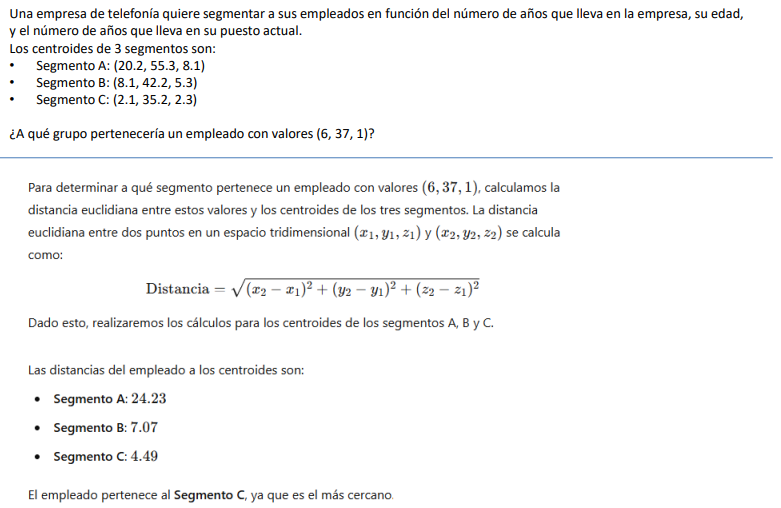
\includegraphics[width=0.95\linewidth]{imagenes/examen-clustering1.png}
    \label{fig:examen-clustering1}
\end{figure}


\begin{figure}[ht]
    \centering
    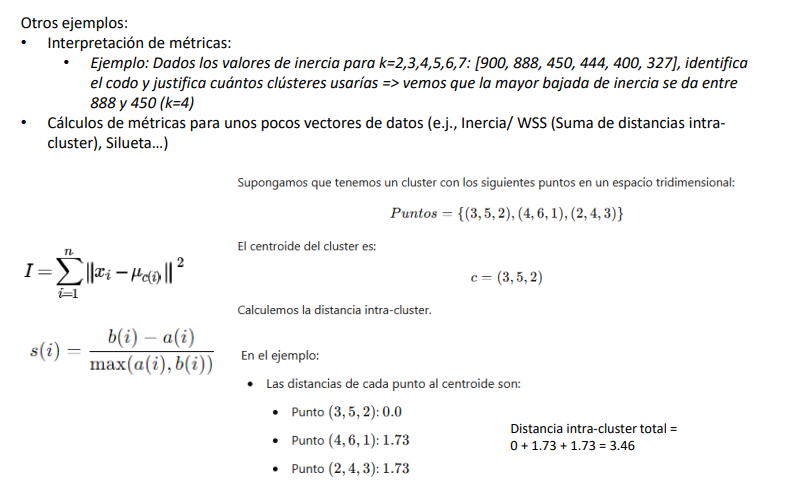
\includegraphics[width=0.95\linewidth]{imagenes/examen-clustering2.png}
    \label{fig:examen-clustering2}
\end{figure}